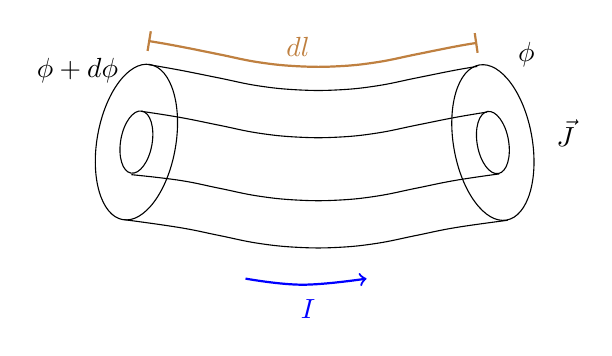
\begin{tikzpicture}

\draw [rotate=-10] (-2.7709,1.0204) node (v1) {} ellipse (0.5 and 1);
\draw   [rotate=10](2.2025,1.115) ellipse (0.5 and 1);
\draw   [rotate=-10](v1) ellipse (0.2 and 0.4);
\draw  [rotate=10] (2.2025,1.115) ellipse (0.2 and 0.4);
\draw  plot[smooth, tension=.7] coordinates {(-2.4034,2.471) (-2,2.4) (-1.5,2.3) (-1,2.2) (-0.4929,2.1489) (0.0071,2.1489) (0.5,2.2) (1,2.3) (1.5,2.4) (1.777,2.4468)};
\draw  plot[smooth, tension=.7] coordinates {(-2.4905,1.8771) (-2,1.8) (-1.5,1.7) (-1,1.6) (-0.4929,1.5489) (0.0071,1.5489) (0.5,1.6) (1,1.7) (1.5,1.8) (1.9027,1.8675)};
\draw  plot[smooth, tension=.7] coordinates {(-2.6162,1.0725) (-2,1) (-1.5,0.9) (-1,0.8) (-0.4929,0.7489) (0.0071,0.7489) (0.5,0.8) (1,0.9) (1.5,1) (2.0573,1.0822)};
\draw  plot[smooth, tension=.7] coordinates {(-2.7,0.5) (-2,0.4) (-1.5,0.3) (-1,0.2) (-0.4929,0.1489) (0.0071,0.1489) (0.5,0.2) (1,0.3) (1.5,0.4) (2.1637,0.4932)};
\draw [->, blue, thick] plot[smooth, tension=.7] coordinates {(-1.1661,-0.2477) (-0.4411,-0.3251) (0.3709,-0.2477)};
\node at (-0.3735,-0.6344) [blue]{$I$};
\node at (-3.3,2.4) {$\phi +d\phi$};
\node at (2.4,2.6) { $\phi$};
\draw [|-|, thick, brown] plot[smooth, tension=.7] coordinates {(-2.4034,2.771) (-2,2.7) (-1.5,2.6) (-1,2.5) (-0.4929,2.4489) (0.0071,2.4489) (0.5,2.5) (1,2.6) (1.5,2.7) (1.777,2.7468)};

\node at (-0.5,2.7) [brown]{$dl$};
\node at (2.9,1.6) {$\vec{J}$};
\end{tikzpicture}